% ============================================================
%  IGNITION SCADA — COURSE SYLLABUS / SELL SHEET
% ============================================================
\documentclass[10pt]{article}
\usepackage[T1]{fontenc}
\usepackage[utf8]{inputenc}
\usepackage{lmodern}
\usepackage{microtype}
\usepackage{palatino}
\usepackage[scaled=0.82]{beramono}
\usepackage[top=0.55in, bottom=0.55in, left=0.65in, right=0.65in]{geometry}
\usepackage[dvipsnames,svgnames,x11names]{xcolor}
\usepackage{tikz}
\usetikzlibrary{positioning,shapes.geometric,arrows.meta,calc,backgrounds,fit}
\usepackage{booktabs}
\usepackage{array}
\usepackage{enumitem}
\usepackage[most]{tcolorbox}
\usepackage[colorlinks=true, linkcolor=oblue, urlcolor=ocyan,
  pdftitle={Ignition SCADA — Course Syllabus}]{hyperref}
\usepackage{parskip}

\definecolor{oblue}{HTML}{C2410C}
\definecolor{ocyan}{HTML}{EA580C}
\definecolor{onavy}{HTML}{431407}
\definecolor{oyellow}{HTML}{D97706}
\definecolor{ogreen}{HTML}{15803D}
\definecolor{oaccent}{HTML}{FFF7ED}
\definecolor{ogray}{HTML}{6B7280}

\setlength{\parskip}{3pt}
\setlength{\parindent}{0pt}
\pagestyle{empty}

\begin{document}

\begin{tikzpicture}[remember picture, overlay]
  \fill[onavy] (current page.north west) rectangle ([yshift=-1.05in]current page.north east);
  \node[anchor=west, text=white, font=\fontsize{22}{26}\bfseries\sffamily]
    at ([xshift=0.65in, yshift=-0.38in]current page.north west) {Ignition SCADA};
  \node[anchor=west, text=ocyan!80, font=\fontsize{11}{13}\sffamily]
    at ([xshift=0.65in, yshift=-0.68in]current page.north west) {Study Guide · Industrial Automation Series · SCADA Hub Training Platform};
  \node[anchor=east, draw=ocyan, rounded corners=5pt, fill=oblue!60,
        inner sep=6pt, text=white, font=\small\bfseries\sffamily]
    at ([xshift=-0.65in, yshift=-0.38in]current page.north east)
    {10 Chapters · 200+ Questions · PDF Included};
  \draw[oyellow, line width=2pt]
    ([xshift=0.65in, yshift=-0.88in]current page.north west) --
    ([xshift=3.5in, yshift=-0.88in]current page.north west);
\end{tikzpicture}

\vspace{0.95in}

\begin{minipage}[t]{0.60\textwidth}

{\color{onavy}\rule{\linewidth}{1.2pt}}
\smallskip
{\small\sffamily\color{ogray}\MakeUppercase{What This Course Teaches}}
\smallskip

Ignition by Inductive Automation is the fastest-growing SCADA platform in North America. Its unlimited licensing model (one server license, unlimited clients, unlimited tags) has disrupted a market where the incumbent pricing model charged per tag and per seat. Ignition runs on standard Linux or Windows hardware, uses an open database backend, delivers HMI via web browser without plugins, and integrates Python scripting natively.

Engineers who know Ignition can build, deploy, and maintain a full SCADA application — tags, alarms, historical data, and multi-site dashboards — faster than any previous generation of SCADA tools allowed. This course covers the complete Ignition stack: Gateway, Designer, Perspective module, Tag Historian, Alarm Notification, and database integration.

\smallskip
{\color{oblue}\rule{\linewidth}{0.6pt}}
\smallskip
{\small\sffamily\color{ogray}\MakeUppercase{Chapter Sequence}}

\setlist[enumerate]{noitemsep, topsep=2pt, leftmargin=*, label=\textcolor{oblue}{\small\bfseries\arabic*.}}
\begin{enumerate}\small
  \item \textbf{Gateway Architecture} — Installation, module system, Gateway web interface, backup/restore, redundancy configuration.
  \item \textbf{Tag System} — OPC tags, expression tags, memory tags, derived tags, tag groups, scan classes, UDTs (User-Defined Types).
  \item \textbf{OPC-UA Integration} — Ignition as OPC-UA server and client, connecting to Siemens, Allen-Bradley, Modbus devices.
  \item \textbf{Perspective Module} — Component library, View/Page/Session architecture, binding system, mobile-responsive design.
  \item \textbf{Scripting} — Python 2.7 (Jython) runtime, system library, tag event scripts, gateway event scripts, scheduled scripts.
  \item \textbf{Alarm Notification} — Alarm modes, pipelines, escalation, acknowledgment, roster configuration, email/SMS notification.
  \item \textbf{Tag Historian} — Storage providers, partitioning, aggregation modes, SPE (Store and Forward), reporting queries.
  \item \textbf{Database Integration} — Named queries, Transaction Groups, JDBC drivers, report generation from live and historical data.
  \item \textbf{Security \& Access} — Identity providers, role mapping, project permissions, SSL/TLS configuration, audit logging.
  \item \textbf{Field Lab} — Build a complete SCADA application: PLC $\to$ OPC-UA $\to$ Ignition tags $\to$ Perspective dashboard $\to$ alarm $\to$ historian $\to$ report.
\end{enumerate}

\smallskip
{\color{oblue}\rule{\linewidth}{0.6pt}}
\smallskip

{\small\sffamily\color{ogray}\MakeUppercase{The Story}}

\small Traditional SCADA platforms charged for every tag, every client seat, and every module add-on. A mid-sized plant with 10,000 tags and 20 client seats was a $\$500$k software investment. Ignition changed the economics: one server license, everything included, tags unlimited. The Ignition trial version runs indefinitely in two-hour session resets — meaning any engineer can learn the full platform without a license.

Inductive Automation's certification program (Inductive University, free online) is the fastest growing training program in industrial automation. Ignition knowledge is increasingly a hiring requirement. This course provides the structured foundation that the scattered Inductive University modules assume — with the field-engineer context that online tutorials omit.

\end{minipage}
\hfill
\begin{minipage}[t]{0.36\textwidth}

% Ignition stack diagram
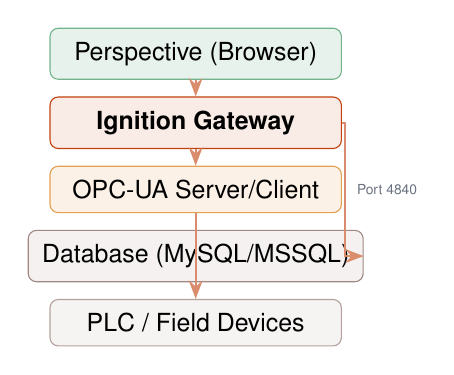
\begin{tikzpicture}[
  layer/.style={rectangle, rounded corners=3pt, draw, fill, text centered,
    font=\small\sffamily, inner sep=5pt, minimum width=3.7cm, minimum height=0.58cm},
  arr/.style={-Stealth, thick, color=oblue!60}
]
\node[layer, draw=ogreen!60, fill=ogreen!10] (client) {Perspective (Browser)};
\node[layer, draw=oblue, fill=oblue!10, below=6pt of client] (gw) {\textbf{Ignition Gateway}};
\node[layer, draw=oyellow!70, fill=oyellow!10, below=6pt of gw] (opc) {OPC-UA Server/Client};
\node[layer, draw=onavy!50, fill=onavy!6, below=6pt of opc] (db) {Database (MySQL/MSSQL)};
\node[layer, draw=onavy!40, fill=onavy!5, below=6pt of db] (plc) {PLC / Field Devices};

\draw[arr] (client) -- (gw);
\draw[arr] (gw) -- (opc);
\draw[arr] (gw) -- ++(1.9cm, 0) |- (db);
\draw[arr] (opc) -- (plc);

\node[font=\tiny\sffamily\color{ogray}, right=2pt of opc] {Port 4840};
\end{tikzpicture}

\vspace{5pt}

\begin{tcolorbox}[
  enhanced, colback=oaccent, colframe=oblue, arc=4pt,
  fonttitle=\small\bfseries\sffamily\color{white},
  title=Certification Relevance,
  boxed title style={colback=oblue},
  attach boxed title to top left={yshift=-2mm, xshift=5mm},
  top=8pt, bottom=6pt, left=6pt, right=6pt
]
\setlist[itemize]{noitemsep, topsep=0pt, leftmargin=*, label=\textcolor{oblue}{$\bullet$}}
\begin{itemize}\small
  \item \textbf{Inductive University Certified} — Core, Advanced, and Gold exams; free, self-paced, industry-recognized.
  \item \textbf{ISA CCST} — SCADA system configuration, alarming, and historian concepts are tested.
  \item \textbf{Ignition Integrator Certification} — Required for Inductive Automation Certified Integrators; demonstrates full-stack project capability.
\end{itemize}
\end{tcolorbox}

\vspace{5pt}

\begin{tcolorbox}[
  enhanced, colback=oyellow!8, colframe=oyellow, arc=4pt,
  fonttitle=\small\bfseries\sffamily\color{white},
  title=Next Steps (Certs),
  boxed title style={colback=oyellow},
  attach boxed title to top left={yshift=-2mm, xshift=5mm},
  top=8pt, bottom=6pt, left=6pt, right=6pt
]
\begin{enumerate}[noitemsep, topsep=0pt, leftmargin=*, label=\small\textcolor{oyellow!80!black}{\arabic*.}]
  \item \small Download Ignition trial from \texttt{inductiveautomation.com} (free, unlimited resets).
  \item Complete Inductive University Core certification (free, online, approximately 20 hours).
  \item Build a complete project from scratch using the lab chapter as a guide.
  \item Pursue Gold certification for the Certified Integrator pathway.
\end{enumerate}
\end{tcolorbox}

\vspace{3pt}

\begin{center}
\begin{tikzpicture}
  \foreach \val/\lbl/\col [count=\i] in {
    10/Chapters/oblue,
    200+/Questions/oyellow,
    Free/Trial/ogreen
  }{
    \node[rectangle, rounded corners=3pt, fill=\col!12, draw=\col!40,
          inner sep=5pt, minimum width=1.1cm, font=\sffamily, text=\col] at (\i*1.35, 0)
      {\textbf{\val}\\\tiny\color{ogray}\lbl};
  }
\end{tikzpicture}
\end{center}

\end{minipage}

\begin{tikzpicture}[remember picture, overlay]
  \fill[onavy!90] (current page.south west) rectangle ([yshift=0.32in]current page.south east);
  \node[anchor=west, text=white!70, font=\footnotesize\sffamily]
    at ([xshift=0.65in, yshift=0.16in]current page.south west)
    {SCADA Hub Training Platform · scada-hub.vercel.app · Free access · No account required for study material};
  \node[anchor=east, text=ocyan, font=\footnotesize\bfseries\sffamily]
    at ([xshift=-0.65in, yshift=0.16in]current page.south east)
    {Course 7 of 8};
\end{tikzpicture}

\end{document}
